\documentclass[hyperref={unicode=true}]{beamer}

\usepackage[russian]{babel}
\usepackage[warn]{mathtext}
\usepackage[utf8]{inputenc}

%\usepackage{fontspec}
%\newfontfamily\cyrillicfont[Script=Cyrillic]{Times New Roman}
%\newfontfamily\cyrillicfontsf[Script=Cyrillic]{Arial}
%\newfontfamily\cyrillicfonttt[Script=Cyrillic]{Courier New}
%\usepackage{polyglossia}
\usepackage{minted}
\usepackage{scrextend}

\usetheme{Boadilla}
\usecolortheme{whale}
\uselanguage{Russian}
\languagealias{russian}{Russian}

\usepackage{wrapfig}
\title{Shell practice}
\author{Воробьёв Станислав}
\date{\today\\[2em]
	Для начала:\\
	\texttt{git clone https://github.com/vissi/shell-supplement.git}
}

\begin{document}

\frame{\titlepage}

%\section*{План}

%\frame{\tableofcontents}

%\section{Введение}

\frame
{
	\frametitle{Откуда есть пошел shell}
	UNIX!
    \begin{columns}[T]
	\column{0.5\textwidth}
	\begin{itemize}
		\item 1971: Thompson
			\begin{itemize}
				\item pipes (McIlroy)
			\end{itemize}
		\item 1975: Mashey
		\item 1977: \texttt{bash} (Bourne)
		\item 1978: \texttt{csh} (Joy)
		\begin{itemize}
			\item 1989: \texttt{tcsh}
		\end{itemize}
		\item 1983: \texttt{ksh} (Korn)
		\item 1989: \texttt{ash} (Almquist)
		\begin{itemize}
			\item 2001: \texttt{busybox}
		\end{itemize}
		\item 1989: \texttt{rc} (Duff) (\textit{Plan~9})
		\begin{itemize}
			\item 1992: \texttt{es} (Rakitzis, Haahr)
		\end{itemize}
		\item 1990: \texttt{zsh} (Falstad)
	\end{itemize}
	\column{0.5\textwidth}
    \begin{itemize}
		\item Thompson shell: \url{http://v6shell.org/}
		\item Plan~9 from~User Space: \url{swtch.com/plan9port/}
		\item Plan~9: \url{plan9.bell-labs.com}
    \end{itemize}
	\end{columns}
}

\begin{frame}
	\frametitle{Commands}
	Control:
	\begin{itemize}
		\item \texttt{find, xargs, expr}
		\item \texttt{less, tee, cat, dd}
	\end{itemize}
	Text processing:
	\begin{itemize}
		\item \texttt{sort, uniq, cut, tr, paste, join, head, tail, grep}
		\item \texttt{zcat, bzgrep, pgrep, ngrep, git grep}
		\item \texttt{sed, awk, perl}
		\item \texttt{lex, bison}
	\end{itemize}
	Files:
	\begin{itemize}
		\item \texttt{ls, touch, file}
		\item \texttt{which, whereis, locate}
		\item \texttt{strings, diff}
	\end{itemize}
	Net:
	\begin{itemize}
		\item \texttt{ssh, scp, rsync}
		\item \texttt{dig, nmap, whois, traceroute}
	\end{itemize}
\end{frame}

\begin{frame}[fragile]
	\frametitle{bash operators}
	\begin{minted}{bash}
SumLines() {
    local sum=0
    local line=""
    while read line ; do
        sum=$((${sum} + ${line}))
    done
    echo ${sum}
}

if [[ -e file.txt ]]; then
    echo file exists
fi
case $t in
abc*)  <action> ;;
esac
	\end{minted}
\end{frame}

\begin{frame}[fragile]
	\frametitle{find, xargs}
    find:
	\begin{addmargin}[1em]{0em}
	\begin{minted}{bash}
    $ find ~/ -name '*.txt' \
        -maxdepth 2 \
        -ctime 1 \   # days
        -cmin  60 \  # minutes
        -iname '*.TXT' \
        -size +1M \
        -type f \ # 'd' for directory
        -not -empty

    $ find ~/ -name '*.txt' -or -name '*.csv'
	\end{minted}
	\end{addmargin}

    xargs:
	\begin{addmargin}[1em]{0em}
	\begin{minted}{bash}
    $ find ~/ -type f -print0 \
        | xargs -0 grep -liwZ GUI \
        | xargs -0 rm -f
    $ grep -rliwZ GUI ~/ | xargs -0 rm -f
	\end{minted}
	\end{addmargin}

\end{frame}

\begin{frame}[fragile]
    \frametitle{xargs, expr}
    xargs:
	\begin{addmargin}[1em]{0em}
	\begin{minted}{bash}
    $ ls *gif | xargs -t -n1 -P2 gif2png
    # -t    Print command to stderr.
    # -n1   At most 1 argument per command line.
    # -P2   Run up to 2 processes simultaneously.
	\end{minted}
	\end{addmargin}
    expr:
    \begin{columns}[T]
	\column{0.3\textwidth}
        \begin{minted}{bash}
        $ expr 3 + 5
        8
        $ expr 5 % 3
        2
        \end{minted}

	\column{0.3\textwidth}
        \begin{minted}{bash}
        $ expr 5 \* 3
        15
        $ y=`expr $y + 1`
        \end{minted}
	\end{columns}

    \vspace{.5em}
    \begin{addmargin}[1em]{0em}
    \begin{minted}{bash}
    $ expr 1 / 0
    expr: division by zero
    Illegal arithmetic operations not allowed.
    $ z=`expr substr $string $position $length`
	\end{minted}
	\end{addmargin}
\end{frame}

\begin{frame}[fragile]
	\frametitle{Control}

	rm core dumps:
	\begin{addmargin}[1em]{0em}
	\begin{minted}{bash}
		find ~/ -name 'core*' -exec rm {} \;
	\end{minted}
	\end{addmargin}

	find config IPs:
	\begin{addmargin}[1em]{0em}
	\begin{minted}{bash}
		m='[0-9][0-9]*';mask="$m[.]$m[.]$m[.]$m";dn=/dev/null
		$ find /etc -exec grep -HnI $mask {} 2>$dn \; | head -n 1
		/etc/mysql/my.cnf:47:bind-address = 127.0.0.1
	\end{minted}
	\end{addmargin}

	find config containing 'listen' word:
	\begin{addmargin}[1em]{0em}
	\begin{minted}{bash}
		$ find . -name "*.conf" | xargs grep "listen"
		./puppet/modules/sphinx/files/sphinx.conf: listen = 9312
	\end{minted}
	\end{addmargin}

	list processes:
	\begin{addmargin}[1em]{0em}
	\begin{minted}{bash}
		ps h | awk '{print $1}' | xargs -I '{}' sh -c \
		'test -f /proc/{}/status && \
			(echo -n {}; head -n 1 /proc/{}/status | cut -c 5-)'
	\end{minted}
	\end{addmargin}
\end{frame}

\begin{frame}[fragile]
	\frametitle{bash}
	sort:
	\begin{addmargin}[1em]{0em}
		\begin{minted}{bash}
		$ sort testfile | uniq -c | sort -nr
		2 word1
		1 word2
		\end{minted}
	\end{addmargin}

	sequential process:
	\begin{addmargin}[1em]{0em}
		\begin{minted}{bash}
		IFS=","
		orders="1126,5553,2316"
		for v in $orders; do
		    process "$v"
		done
		# seq=`perl -e "\$,=' ';print 2..$max"`
		for v in `seq 1 3`; do echo $v; done
		\end{minted}
	\end{addmargin}

	parallel:
	\begin{addmargin}[1em]{0em}
		\begin{minted}{bash}
	find . -type f | parallel -k grep -H -n $1 {}
		\end{minted}
	\end{addmargin}
	mapreduce:
	\begin{itemize}
		\item \url{https://github.com/erikfrey/bashreduce}
	\end{itemize}
\end{frame}


\begin{frame}[fragile]
	history optimization:
	\begin{addmargin}[1em]{0em}
		\begin{minted}{bash}
$ p='{ cnt[$0]++ } END { for (i in cnt) print cnt[i], i }'
$ history \
    | sed 's/^ \+//;s/  / /' \
    | cut -d' ' -f2- \
    | awk $p | sort -rnk 1 | head -n 10
416 ls
347 gst
101 ssh vissi.su 
99 cd ~
86 cd ..
47 git diff 
41 sudo service nginx start
37 v ../index.html
34 v test.php
32 git pull 
		\end{minted}
	\end{addmargin}

\end{frame}

\begin{frame}[fragile]
	\frametitle{Text: encoding}
	%\begin{figure}
		\begin{center}
			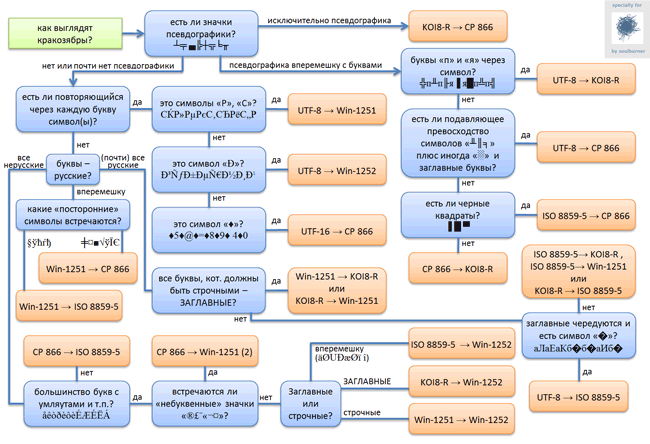
\includegraphics[width=230pt]{encoding.png}
			\vspace{12pt}
			\begin{minted}{bash}
				$ enca docs/workflow.md -L russian
				Universal transformation format 8 bits; UTF-8
				$ iconv -f CP1251 -t UTF-8
			\end{minted}
		\end{center}
		%\caption{...}
	%\end{figure}
\end{frame}

\begin{frame}[fragile]
	\frametitle{sed}
	\begin{itemize}
		\item sed~--- \textbf{s}tream \textbf{ed}itor
		\item Lee E. McMahon, 1973
        \item \url{http://www.opennet.ru/base/dev/sed1line.txt.html}
	\end{itemize}

	\begin{addmargin}[1em]{0em}
	\begin{minted}{bash}
    $ sed 's/1/5/g'
    \end{minted}
	\end{addmargin}

    word frequency:
	\begin{addmargin}[1em]{0em}
	\begin{minted}{bash}
    $ cat "$1" | xargs -n1 | \
    # List the file, one word per line.
    tr A-Z a-z | \
    #  Shift characters to lowercase.
    sed -e 's/\.//g'  -e 's/\,//g' -e 's/ //g' | \
    # Filter out periods and commas, and
    # change space between words to linefeed,
    sort | uniq -c | sort -nr
    # Finally remove duplicates, prefix occurrence count
    # and sort numerically.
    \end{minted}
	\end{addmargin}
\end{frame}

\begin{frame}[fragile]
	\frametitle{awk}
	\begin{itemize}
		\item awk~--- язык разбора записей по шаблону
		\item Alfred~V.~\textbf{A}ho, Peter~J.~\textbf{W}einberger и Brian~W.~\textbf{K}ernighan (1977)
		\item Тьюринг-полный
			\begin{itemize}
				\item \url{https://github.com/darius/awklisp}
			\end{itemize}
	\end{itemize}

	Программа имеет три секции:

	\begin{addmargin}[1em]{0em}
		\begin{minted}{awk}
			BEGIN { } # before
			/pattern/ { print "$1" } # for each matching line
			# ...
			END   { } # after
		\end{minted}
	\end{addmargin}

		\texttt{wc}:
	\begin{addmargin}[1em]{0em}
		\begin{minted}{awk}
			{ total = total + NF }; END {print total}
		\end{minted}
	\end{addmargin}

	\texttt{head}:
	\begin{addmargin}[1em]{0em}
		\begin{minted}{awk}
			NR < 11
		\end{minted}
	\end{addmargin}
\end{frame}

\begin{frame}[fragile]
	\frametitle{awk}
	range:
	\begin{addmargin}[1em]{0em}
		\begin{minted}{awk}
			awk 'NR==8,NR==12'
		\end{minted}
	\end{addmargin}

	multiple files:
	\begin{addmargin}[1em]{0em}
		\begin{minted}{awk}
		awk 'FNR==1{print}' file1 file2
		\end{minted}
	\end{addmargin}

	gawk networking:
	\begin{addmargin}[1em]{0em}
		\begin{minted}{awk}
BEGIN {
   RS = ORS = "\r\n"
   HttpService = "/inet/tcp/0/google.com/80"
   print "GET http://google.com"     |& HttpService
   while ((HttpService |& getline) > 0)
      print $0
   close(HttpService)
}
		\end{minted}
	\end{addmargin}
\end{frame}

\begin{frame}[fragile]
    \frametitle{awk, join}
	\begin{itemize}
        \item \url{http://www.pement.org/awk/awk1line.txt}
	\end{itemize}
    excel:
	\begin{addmargin}[1em]{0em}
		\begin{minted}{awk}
        $ join \
            <(awk '{print $1, $2 + $3}') \
            <(awk '{print $1, substr($2,1,3)}')

        $ awk '$5 == "abc123"'
        $ awk '$7  ~ /^[a-f]/'
        # concat
        $ awk 'ORS=NR%2?",":"\n"'
		\end{minted}
	\end{addmargin}
\end{frame}

\begin{frame}[fragile]
	\frametitle{zsh}

	globbing:
	\begin{addmargin}[1em]{0em}
		\begin{minted}{bash}
			rm *.[ch]
			ls -l **/*.log # recursive
			zmv '(*).html' 'template_$1.tmpl'
		\end{minted}
	\end{addmargin}

	autocomplete:
	\begin{addmargin}[1em]{0em}
		\begin{minted}{bash}
			$ cd /u/l/b
			$ cd /usr/local/bin
			$ cd bin share
			$ pwd
			/usr/local/share
		\end{minted}
	\end{addmargin}

	typo correct:
	\begin{addmargin}[1em]{0em}
		\begin{minted}{bash}
		$ sl
		zsh: correct 'sl' to 'ls' [nyae]?
		\end{minted}
	\end{addmargin}
	% старый баш?
	% http://www.chodorowski.com/projects/zws/
\end{frame}

\begin{frame}[fragile]
	\frametitle{json}
	json (\url{http://stedolan.github.io/jq/}):
	\begin{addmargin}[1em]{0em}
		\begin{minted}{bash}
		$ echo '{"foo": 42, "bar": "more data"}' > foo.json
		$ <foo.json jq '.foo'
		42
		\end{minted}
	\end{addmargin}

	json (\texttt{npm install json}):
	\begin{addmargin}[1em]{0em}
		\begin{minted}{bash}
$ curl -s https://api.github.com/repos/joyent/node/issues \
	| json -a comments number title  -C | sort -n  | tail -2
2	7433	test: add test-spawn-cmd-named-pipe
1	7432	test: relax test-vm-infinite-recursion

$ cat config.json | json
json: error: input is not JSON: Unexpected ',' at line 17, ...
   , { "name": "smartos64-1.4.7"
$ echo $?
1
		\end{minted}
	\end{addmargin}
\end{frame}

\begin{frame}[fragile]
	\frametitle{xml}
	xml:
	\begin{addmargin}[1em]{0em}
		\begin{minted}{xml}
<xml>
  <table>
    <rec id="1">
      <externalId>123</externalId>
      <paymentAmount>100.00</paymentAmount>
      <paymentCurrency>RUB</paymentCurrency>
    </rec>
</xml>
		\end{minted}
	\end{addmargin}

	\texttt{xmlstarlet}:
	\begin{addmargin}[1em]{0em}
		\begin{minted}{bash}
$ xml el table.xml
xml
xml/table
xml/table/rec
xml/table/rec/paymentAmount
xml/table/rec/paymentCurrency
		\end{minted}
	\end{addmargin}
\end{frame}

\begin{frame}[fragile]
	\frametitle{binary}
	\begin{addmargin}[1em]{0em}
		\begin{minted}{bash}
$ hexdump -v -e '"%010_ad  |" 8/1 "%02X "' \
	-e '"|" 8/1 "%_p" "|\n"' pdt_deploy_target.sh | head -n 2
0000000000  |23 21 2F 62 69 6E 2F 73|#!/bin/s|
0000000008  |68 0A 23 20 75 73 65 20|h.# use |

$ xxd -c 8 pdt.sh | head -n 2
0000000: 2321 2f62 696e 2f73  #!/bin/s
0000008: 680a 2320 7573 6520  h.# use 

$ xxd pdt.sh | head -n 2 | xxd -r | head -n 2
#!/bin/sh
# use it as gist?
		\end{minted}
	\end{addmargin}
\end{frame}

\begin{frame}[fragile]
	\frametitle{vim}
	quickstart:
	\begin{addmargin}[1em]{0em}
		\begin{minted}{vim}
			sy on
			set ai
			set number
		\end{minted}
	\end{addmargin}

	goto:
	\begin{addmargin}[1em]{0em}
		\begin{minted}{bash}
			$ vim +47 FileWithError.php
		\end{minted}
	\end{addmargin}

	invoke shell:
	\begin{addmargin}[1em]{0em}
		\begin{minted}{vim}
			:sh
			:make
			:!./run-tests.sh
		\end{minted}
	\end{addmargin}

	save w/ sudo:
	\begin{addmargin}[1em]{0em}
		\begin{minted}{vim}
			:w !sudo tee % >/dev/null
		\end{minted}
	\end{addmargin}

	\texttt{.vimrc}:
	\begin{addmargin}[1em]{0em}
		\begin{minted}{vim}
			cnoremap sudow w !sudo tee % >/dev/null
		\end{minted}
	\end{addmargin}

	encoding:
	\begin{addmargin}[1em]{0em}
		\begin{minted}{vim}
			:e ++enc=cp1251
		\end{minted}
	\end{addmargin}
\end{frame}

\begin{frame}[fragile]
	\frametitle{}
	%\begin{figure}
		\begin{center}
			
\includegraphics[width=240pt]{python.jpg}
			\vspace{12pt}
		\end{center}
		%\caption{...}
	%\end{figure}
\end{frame}

\begin{frame}[fragile]
	\frametitle{misc}

	\texttt{tcc} script:
	\begin{addmargin}[1em]{0em}
		\begin{minted}{c}
#!/usr/bin/tcc -run
#include <cstdio>
int main(int argc, char** argv) {
    printf("%s\n", "hello, world!");
    return 0;
}
		\end{minted}
	\end{addmargin}

	\texttt{scsh} script:
	\begin{addmargin}[1em]{0em}
		\begin{minted}{scheme}
#!/usr/local/bin/scsh -s
!#
(define (exf dir)
  (with-cwd dir
    (filter file-executable? (directory-files dir #t))))
(define (writeln x) (display x) (newline))
(for-each writeln
  (append-map exf ((infix-splitter ":") (getenv "PATH"))))
		\end{minted}
	\end{addmargin}
\end{frame}

\frame
{
	\frametitle{Вопросы}
	
	\begin{center}
	Вопросы?\\
	\vspace{15pt}
	\textit{vim | UNIX | Cybernetics} ?\\
	\vspace{15pt}
	\url{http://vissi.su/links/unix/}\\
	\vspace{25pt}
	Спасибо!
	\end{center}

}

\end{document}
